\documentclass[xcolor=x11names,compress]{beamer}

%% General document %%%%%%%%%%%%%%%%%%%%%%%%%%%%%%%%%%
\usepackage{graphicx}
\usepackage{tikz}
\usepackage{Tabbing}
\usetikzlibrary{decorations.fractals}
\usepackage{fancyvrb}
\usepackage{verbatim}
%%%%%%%%%%%%%%%%%%%%%%%%%%%%%%%%%%%%%%%%%%%%%%%%%%%%%%

%% Beamer Layout %%%%%%%%%%%%%%%%%%%%%%%%%%%%%%%%%%
\useoutertheme[subsection=false,shadow]{miniframes}
\useinnertheme{default}
\usefonttheme{serif}
\usepackage{palatino}
\usepackage{tabu}
% Links
\usepackage{hyperref}
\definecolor{links}{HTML}{003262}
\hypersetup{colorlinks,linkcolor=,urlcolor=links}

% addition of color
\usepackage{xcolor}
\definecolor{CoolBlack}{rgb}{0.0, 0.18, 0.39}
\definecolor{byellow}{rgb}{0.55037, 0.38821, 0.06142}
\definecolor{dgreen}{rgb}{0.,0.6,0.}
\definecolor{RawSienna}{cmyk}{0,0.72,1,0.45}
\definecolor{forestgreen(web)}{rgb}{0.13, 0.55, 0.13}
\definecolor{cardinal}{rgb}{0.77, 0.12, 0.23}

\setbeamerfont{title like}{shape=\scshape}
\setbeamerfont{frametitle}{shape=\scshape}

\setbeamercolor*{lower separation line head}{bg=CoolBlack}
\setbeamercolor*{normal text}{fg=black,bg=white}
\setbeamercolor*{alerted text}{fg=dgreen} % just testing; I think this looks better
\setbeamercolor*{example text}{fg=black}
\setbeamercolor*{structure}{fg=black}

\setbeamercolor*{palette tertiary}{fg=black,bg=black!10}
\setbeamercolor*{palette quaternary}{fg=black,bg=black!10}

% Margins
\usepackage{changepage}

\mode<presentation>
{
  \definecolor{berkeleyblue}{HTML}{003262}
  \definecolor{berkeleygold}{HTML}{FDB515}
  \usetheme{Boadilla}      % or try Darmstadt, Madrid, Warsaw, Boadilla...
  %\usecolortheme{dove} % or try albatross, beaver, crane, ...
  \setbeamercolor{structure}{fg=berkeleyblue,bg=berkeleygold}
  \setbeamercolor{palette primary}{bg=berkeleyblue,fg=white} % changed this
  \setbeamercolor{palette secondary}{fg=berkeleyblue,bg=berkeleygold} % changed this
  \setbeamercolor{palette tertiary}{bg=berkeleyblue,fg=white} % changed this
  \usefonttheme{structurebold}  % or try serif, structurebold, ...
  \useinnertheme{circles}
  \setbeamertemplate{navigation symbols}{}
  \setbeamertemplate{caption}[numbered]
  \usebackgroundtemplate{}
}


\usepackage{cutwin}

% adding slide numbers
\addtobeamertemplate{navigation symbols}{}{%
    \usebeamerfont{footline}%
    \usebeamercolor[fg]{footline}%
    \hspace{1em}%
    \insertframenumber/\inserttotalframenumber
}

% equation stuff
\usepackage{mathrsfs}
\usepackage[mathcal]{euscript}
\usepackage{amssymb}
\usepackage{amsthm}
\usepackage{epsfig}
\usepackage{amsmath}

% title stuff for footer
\title{Binary Formulation of Decay Equations}
\author{Scopatz, Bates, Wilson}
\date{LANL-XX-XXXX}

% arrow
\usetikzlibrary{shapes.arrows}
\tikzset{
        myarrow/.style={
        draw,
        fill=orange,
        single arrow,
        minimum height=3.5ex,
        single arrow head extend=0.5ex}
}

\newcommand{\arrowdown}{
 \tikz [baseline=-1ex]{\node [myarrow,rotate=-90] {};}
}

%%%%%%%%%%%%%%%%%%%%%%%%%%%%%%%%%%%%%%%%%%%%%%%%%%%%%
\begin{document}



%%%%%%%%%%%%%%%%%%%%%%%%%%%%%%%%%%%%%%%%%%%%%%%%%%%%%%
%%%%%%%%%%%%%%%%%%%%%%%%%%%%%%%%%%%%%%%%%%%%%%%%%%%%%%
\begin{frame}
\title{Binary Formulation of Decay Equations}
%\subtitle{}
\author{\textbf{Cameron~R.~Bates$^{2}$} for Anthony~Scopatz$^{1}$ \\
        \vspace{0.1in}
        Paul Wilson$^{1}$\\
        \vspace{0.1in}
        $^{1}$ The University of Wisconsin-Madison\\
        $^{2}$ Los Alamos National Laboratory}

\date{ANS Summer Meeting, June, 2015}
\titlepage
\end{frame}

%------------------------------------------------------
\begin{frame}{Outline}
    \Large
	\begin{columns}
  	\begin{column}{0.5\textwidth}
	    \begin{itemize}
        \item Motivation
        \item Method Derivation
        \item Implementation
	    \end{itemize}
  	\end{column}
 	%
 	\begin{column}{0.4\textwidth}
 	   \begin{center}
 	   \begin{figure}
       
\includegraphics[height=4cm]{pyne-icon-big.png}
	   \end{figure}
 	   \end{center}
  	\end{column}
	\end{columns}

\end{frame}

%%%%%%%%%%%%%%%%%%%%%%%%%%%%%%%%%%%%%%%%%%%%%%%%%%%%%%
%%%%%%%%%%%%%%%%%%%%%%%%%%%%%%%%%%%%%%%%%%%%%%%%%%%%%%
\section{Motivation}
\begin{frame}{Motivation}

    There are many situations in which the Bateman equations 
    \cite{bateman1910solution} should be solved for decay channels only, 
    rather than for genric transmutation:
    
    \vspace*{1em}
    \begin{itemize}
        \item Non-reactor components of the nuclear fuel cycle (storage, 
              disposition, transit)
        \item Activation analysis
        \item Dosage calculation
    \end{itemize}

    \vspace*{1em}
    Many solvers of the Bateman equations are not targeted to this reduced 
    use case.

\end{frame}

%%%%%%%%%%%%%%%%%%%%%%%%%%%%%%%%%%%%%%%%%%%%%%%%%%%%%%
\begin{frame}{Motivation}

    Bateman equations solvers for decay-only calculations can be slow because:
    
    \vspace*{1em}
    \begin{itemize}
        \item They perform a full transmutation calculation but with zero
              neutron flux.
        \item They read in data libraries from disk each calculation.
        \item Perform excess floating-point calculations even for decay
              chanels, which also add algorithimc error.
    \end{itemize}

    For example, ORIGEN v2.2 \cite{croff1980origen2} for decay is 
    O($\approx 1$ sec), most of which is I/O.

    \vspace*{1em}
    This does not scale well to large systems, such a fuel cycle with 70k 
    fuel assemblies or reactor dose calculations with 50k volume elements.

\end{frame}

%%%%%%%%%%%%%%%%%%%%%%%%%%%%%%%%%%%%%%%%%%%%%%%%%%%%%%
%%%%%%%%%%%%%%%%%%%%%%%%%%%%%%%%%%%%%%%%%%%%%%%%%%%%%%
\section{Method Derivation}
\begin{frame}{Goal}

    \vspace*{3em}
    Create a decay-only solver for the Bateman equations 
    that is much faster mathematically and algorithimically than current 
    implementations. 

    \vspace*{1em}
    Such a solver will have reduced algorithimic error stemming from fewer 
    FLOPS.
    
\end{frame}

%%%%%%%%%%%%%%%%%%%%%%%%%%%%%%%%%%%%%%%%%%%%%%%%%%%%%%
\begin{frame}{Canonical Bateman Equations for Decay}

\begin{equation}
\label{bm-eq}
N_C(t) = \frac{N_1(0)}{\lambda_C} \cdot \gamma \cdot \sum_{i=1}^C \lambda_i c_{i} e^{-\lambda_i t}
\end{equation}

\begin{equation}
\label{c_i}
c_i = \prod_{j=1,i\ne j}^C \frac{\lambda_j}{\lambda_j - \lambda_i}
\end{equation}

\begin{table}[hbt]
\label{decay-symbol-meaning}
%\caption{Symbol Meaning in Decay Equations}
\begin{tabular}{|l|l|}
\hline
\textbf{Symbol} & \textbf{Meaning} \\
\hline
$C$         & length of the decay chain\\
$i$         & index for ith species, on range [1, C]\\
$j$         & index for jth species, on range [1, C]\\
$t$         & time [seconds]\\
$N_i(t)$    & number density of the ith species at time t\\
$t_{1/2,i}$ & half-life of the ith species\\
$\lambda_i$ & decay constant of ith species, $\ln(2)/t_{1/2,i}$\\
$\gamma$    & total branch ratio for this chain\\
\hline
\end{tabular}
\end{table}
    
\end{frame}

%%%%%%%%%%%%%%%%%%%%%%%%%%%%%%%%%%%%%%%%%%%%%%%%%%%%%%

\begin{frame}{Canonical Bateman Equations for Decay}

    For first (parent) species in a chain:

\begin{equation}
\label{N_C}
N_C(t) = N_1(0) e^{-\lambda_1 t}
\end{equation}

    \vspace*{2em}
    For last (stable child) species in a chain:

\begin{equation}
\label{lim_lam_N_C}
N_{\lambda_C \to 0}(t) = N_1(0)  \gamma \left[1.0 - \sum_{i=1}^{C-1} \left(\prod_{j=1,i\ne j}^{C-1} \frac{\lambda_j}{\lambda_j - \lambda_i} \right) e^{-\lambda_i t} \right]
\end{equation}

\end{frame}

%%%%%%%%%%%%%%%%%%%%%%%%%%%%%%%%%%%%%%%%%%%%%%%%%%%%%%

\begin{frame}{Method Derivation}

    By grouping constants, it is possible to express the Bateman equations 
    as a simple sum of exponentials:

    \begin{equation}
    \label{N_C_bin}
    N_C(t) = N_1(0) \sum_{i=1}^C k_{i} e^{-\lambda_i t}
    \end{equation}

    \vspace*{1em}
    In Equation \ref{N_C_bin}, the coefficients $k_i$ are defined as follows:

    \begin{equation}
    \label{k_i}
    k_i = \frac{\gamma}{\lambda_C} \lambda_i c_i
    \end{equation}

    \vspace*{1em}
    Precomputing the $k_i$, reduces the number of FLOPS per term in the 
    summation from $O(3C+1)$ to $O(4)$.

\end{frame}

%%%%%%%%%%%%%%%%%%%%%%%%%%%%%%%%%%%%%%%%%%%%%%%%%%%%%%

\begin{frame}{Method Derivation}

    Modern processors are inherently binary.

    \vspace*{1em}
    Thus, naively computing $2^x$ is on average about 25\% faster than 
    computing $e^x$ on most architectures.

    \vspace*{1em}
    Note: some processors come with a special instruction for computing 
    $\exp(x)$ as fast (or faster) than $\exp2(x)$. Intel seems to do this with 
    SSE2, when used at compile time.

    \vspace*{1em}
    Recasting the Bateman equations away from the natural exponent to base-2
    yeilds a `binary' reformulation.

\end{frame}

%%%%%%%%%%%%%%%%%%%%%%%%%%%%%%%%%%%%%%%%%%%%%%%%%%%%%%

\begin{frame}{Method Derivation}

    Define a precomputed constant $a_i$ as,

    \begin{equation}
    \label{a_i}
    a_i = \frac{-1}{t_{1/2,i}}
    \end{equation}

    \vspace*{1em}
    Thus, the final form of the binary representation of the Bateman equations 
    are seen here:

    \begin{equation}
    \label{nc_wakka}
    N_C(t) = N_1(0) \sum_{i=1}^C k_{i} \cdot 2^{a_i t}
    \end{equation}

    \vspace*{1em}
    Every term in the sum is $O(3)$ and every operation is native to the 
    instruction set.

\end{frame}

%%%%%%%%%%%%%%%%%%%%%%%%%%%%%%%%%%%%%%%%%%%%%%%%%%%%%%

\begin{frame}{Method Derivation}

    For first (parent) species in a chain:

\begin{equation}
\label{nc_jawakka}
N_C(t) = N_1(0) \cdot 2^{a_1 t}
\end{equation}

    \vspace*{2em}
    For last (stable child) species in a chain:

\begin{equation}
\label{nc_brown_shoes}
N_{\lambda_C \to 0}(t) = N_1(0) \left[1.0 + \sum_{i=1}^{C-1} \lim_{\lambda_C\to 0}(k_{i}) \cdot 2^{a_i t} \right]
\end{equation}

\end{frame}

%%%%%%%%%%%%%%%%%%%%%%%%%%%%%%%%%%%%%%%%%%%%%%%%%%%%%%

\begin{frame}{Method Derivation}

    \begin{itemize}
        \item Relies on completely precomputed $k_i$ and $a_i$.
        \item No I/O since constants are compiled into implementation.
        \item Preserves all physical processes since no assumptions were made 
              aside from the Bateman equations.
        \item Not possible to further reduce number of operations analytically.
    \end{itemize}

\end{frame}

%%%%%%%%%%%%%%%%%%%%%%%%%%%%%%%%%%%%%%%%%%%%%%%%%%%%%%

\begin{frame}{Implementation}

    A refernece implmentation of this method is available through the pyne 
    library \cite{pyne}.

    \vspace*{1em}
    Cyclus \cite{cyclus2015} uses this implementation for nuclear fuel cycle 
    simulation.

    \vspace*{1em}
    Even this implmentation was forced to make certain assumptions in the 
    face of floating point arithmetic for reasons of
    performance, compile-ability, and computability.

\end{frame}

%%%%%%%%%%%%%%%%%%%%%%%%%%%%%%%%%%%%%%%%%%%%%%%%%%%%%%

\begin{frame}{Implementation Assumptions}

    Spontaneous fission chains are not tallied as they 
    lead to an explosion of the total number of chains while contributing to 
    extraordinarily rare branches. For most species the relative error
    induced is $O(<10^{-8})$.  Relatively few and rare nuclides, such as Cm-250, 
    have spontaneous fission branch greater than 5\%.

    \vspace*{1em}
    Decay alphas are not treated as He-4 production.  This can lead to 
    errors that are less than 2\% of the total mass of all chains for a
    nuclide.  

    \vspace*{1em}
    To prevent other sources of floating point error, a nuclide is 
    determined to be stable when $\lambda_i < 10^{-16}$, rather than when 
    $\lambda_i = 0.0$.


\end{frame}

%%%%%%%%%%%%%%%%%%%%%%%%%%%%%%%%%%%%%%%%%%%%%%%%%%%%%%

\begin{frame}{Implementation Assumptions}

    \vspace*{1em}
    For chains longer than length 2, any 
    term whose half-life is less than $10^{-8}$ of the sum of all 
    half-lives in the chain is dropped. This filtering prevents excessive
    calculation from species which do not significantly contribute to 
    end atom fractions. If the filtering causes there to be less than 
    two terms in the summation, then the filtering is turned off and all
    terms are computed.

    \vspace*{1em}
    If a chain has any $\mathrm{NaN}$ decay constants, the chain is rejected.

    \vspace*{1em}
    If a chain has any infinite $k_i$ values, the chain is rejected.

\end{frame}


%%%%%%%%%%%%%%%%%%%%%%%%%%%%%%%%%%%%%%%%%%%%%%%%%%%%%%

\begin{frame}{Comparison to ORIGEN - Speed}

    Run times are fast:
    \vspace*{1em}
    \begin{itemize}
        \item \textbf{ORIGEN v2.2:} O(1+ sec)
        \item \textbf{Binary:} O(5-100 $\mu$sec)
    \end{itemize}

    \vspace*{1em}
    Factor of $10^3$ to $10^6$ speedup.

    \vspace*{1em}
    ORIGEN runtimes likely stem from from excessive I/O. 

    \vspace*{1em}
    The binary timings depend on the number of chains in a decay and 
    timing results include Python round tripping.

\end{frame}

%%%%%%%%%%%%%%%%%%%%%%%%%%%%%%%%%%%%%%%%%%%%%%%%%%%%%%

\begin{frame}{Comparison to ORIGEN - Method}

    Take $x$ as the mass of a species in a material 
    after decay in the binary formulation, and $y$ as the mass of the 
    same species decayed via ORIGEN. Define the relative error as:

    \vspace*{1em}
    \begin{equation}
    \epsilon = \frac{2 \cdot |x - y|}{x + y}, \epsilon \in [0, 2]
    \end{equation}

    \vspace*{1em}
    \textbf{Experiment:} Decay a unit mass of a nuclide whose half-lives 
    in ORIGEN and ENSDF match to within the precision given in the ORIGEN 
    library. Run this decay  for 0.01, 0.1, 1.0, 10, 100 times the half-life 
    of the nuclide. Compare the relative errors.

    \vspace*{1em}
    This generated 2802 nuclide/decay time cases that are on a common basis.

\end{frame}

%%%%%%%%%%%%%%%%%%%%%%%%%%%%%%%%%%%%%%%%%%%%%%%%%%%%%%

\begin{frame}{Comparison to ORIGEN - Carbon Isotopes}

    \vspace*{-1.5em}
    \begin{center}
    \includegraphics[scale=0.4]{decay-relative-error-C12.eps}
    \includegraphics[scale=0.4]{decay-relative-error-C13.eps}
    \end{center}

    \vspace*{-2.5em}
    \begin{center}
    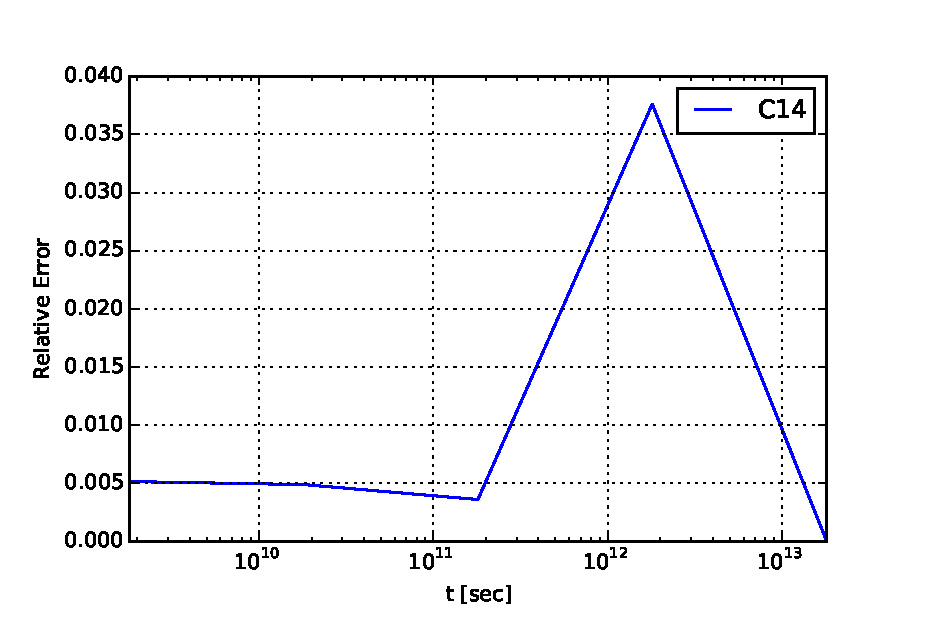
\includegraphics[scale=0.4]{decay-relative-error-C14.eps}
    \includegraphics[scale=0.4]{decay-relative-error-C15.eps}
    \end{center}

\end{frame}

%%%%%%%%%%%%%%%%%%%%%%%%%%%%%%%%%%%%%%%%%%%%%%%%%%%%%%

\begin{frame}{Comparison to ORIGEN - All Cases}

    \begin{center}
    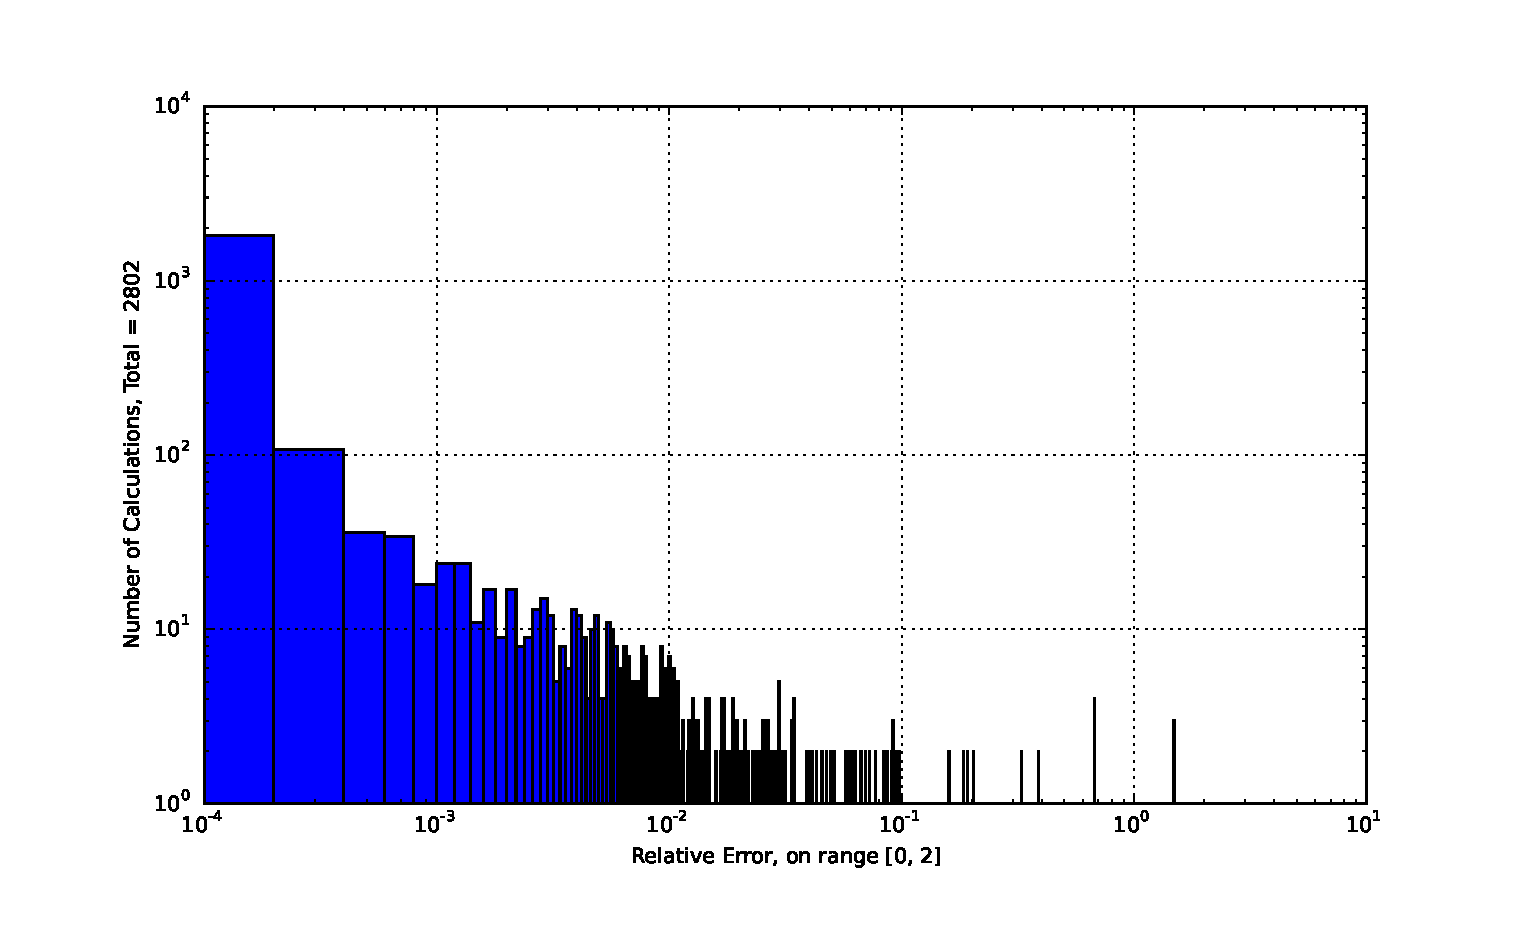
\includegraphics[scale=0.45]{decay-relative-error-histogram.eps}
    \end{center}

    \vspace*{-1em}
    \textbf{Note:} log-log scale to accentuate differences.

\end{frame}

%%%%%%%%%%%%%%%%%%%%%%%%%%%%%%%%%%%%%%%%%%%%%%%%%%%%%%

\section*{}
\begin{frame}[fragile]{Questions?}

    \begin{center}
    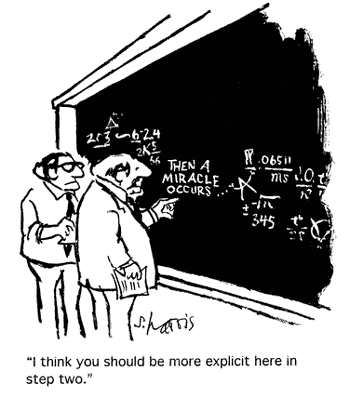
\includegraphics[height=3in,clip]{questions-comic.png}
    \end{center}

\end{frame}

% --------------------------------------------------------------
\begin{frame}[allowframebreaks]{References}
	\bibliographystyle{unsrt}
    \bibliography{ans.bib}
\end{frame}


\begin{comment}


\section{Implementation Specific Approximations}
\label{approx}
The method presented in the previous section has been implemented within
PyNE and Cyclus. However, any given mathematical system of equations
will encounter implementation-specific choices when turned into 
associated software. Thus, though the above formulation holds generally for 
any decay chain, certain approximations have been used in the implementation
for reasons of performance, compile-ability, and computability.
The PyNE implementation generally aims to reduce the number of 
chains and terms that are calculated when they can be shown to be 
redundant or insignificant to the total calculation. In specific, the 
following modeling assumptions have been made:


In principle, each of these statements is reasonable. However, they may 
have covariant effects that inject unreasonable errors into the system.
To ensure that this is not the case for the assumptions above, 
a preliminary benchmark study was performed \cite{benchmark}. This benchmark 
compared
the results of running ORIGEN v2.2 \cite{croff1980origen2} to the results of 
the binary formulation. This study compared 2811 cases for a wide spread of
nuclides over 0.01, 0.1, 1.0, 10, 100 times the half-life of the nuclide.
In the overwhelming majority of cases, the relative errors were found to be 
within acceptable bounds. 
Take $x$ as the mass of a species in a material 
after decay in the binary formulation, and $y$ as the mass of the same species
decayed via ORIGEN, then the relative error $\epsilon$ is computed as:
\begin{equation}
\epsilon = \frac{2 \cdot |x - y|}{x + y}
\end{equation}
For a given nuclide to pass the decay benchmark here, 
the species present in the decayed result must meet the following criteria:
\begin{enumerate}
    \item The highest relative error of any species in the decay result is
          less than 1\%, or

    \item If the species has a relative error greater than 1\%, then the 
          decayed mass of the species multiplied by the relative error
          (the mass-weighted relative error) is less than 10\%.
\end{enumerate}
  
For cases that did demonstrate significant differences in the benchmark, 
the differences could all be traced back to discrepancies in the underling 
data. Since the PyNE binary formulation uses more recent ENSDF decay 
data \cite{bhat1992evaluated} and computes more decay chains than ORIGEN, 
it is reasonable to assume that these discrepancies are not the fault of the 
binary formulation or the implementation assumptions.

It is also important to mention that these implementation assumptions 
may preclude desired behavior by users. For example, perhaps alpha decay 
should be considered He-4 production. This would bring the implementation in
line with the same feature in ORIGEN v2.2. In such a situation, these 
assumptions should be revisited and the implementation should be reworked.

\section{Comparison to ORIGEN implementation}

The implementation of decay calculations in ORIGEN follows a fundamentally 
different strategy from the one described above. It uses Taylor series expansion 
of the exponential decay to make the problem tractable
and then uses run-time branches to make a set of further approximations similar
to those described above. This is due to both the increased scope of the 
problem being solved, transmutation and decay, as well as the design which
treats the decay data and the algorithm as two separate entities. The 
combination of modern computational tools, allowing for efficient generation of 
code, and the existing PyNE decay data interface, with rapid access to up-to-date ENSDF
decay data, enable a merging of the two components and a reduction in computational
cost at run-time with a manageable computation cost at compile (less than 30 seconds on
a modern laptop). 
%%%%%%%%%%%%%%%%%%%%%%%%%%%%%%%%%%%%%%%%%%%%%%%%%%%%%%%%%%%%%%%%%%%%%%%%%%%%%%%%
\section{Conclusions \& Future Work}

Many different computational solutions to the Bateman equations have been 
developed, but few have been focused on optimizing the solution for speed
of implementation without significant approximation of the initial problem.
 The ability to have algorithmically 
generated code makes it possible to generate a solution that is both 
computationally efficient and that minimizes mathematical approximations. This 
work demonstrates such an implementation and shows promising initial results
in comparison to existing tools. It is also unique in that the code requires no
run time access to nuclear data as it is all integrated into the compilation 
process. This results in a single portable C++ file with header that can be 
used in NFC tools for decay calculations. Future work will consist of a more 
detailed benchmark
comparison against existing tools and work to quantify the errors introduced by
the approximations used and those due to other effects such as round-off errors. 

%%%%%%%%%%%%%%%%%%%%%%%%%%%%%%%%%%%%%%%%%%%%%%%%%%%%%%%%%%%%%%%%%%%%%%%%%%%%%%%%
%\section{Acknowledgments}

%%%%%%%%%%%%%%%%%%%%%%%%%%%%%%%%%%%%%%%%%%%%%%%%%%%%%%%%%%%%%%%%%%%%%%%%%%%%%%%%
\bibliographystyle{ans}
\bibliography{bibliography}
\end{document}

\end{comment}

\end{document}



